% !TEX root = ../paper.tex
\section{Interaction techniques} \label{sec:techniques}
Before designing and implementing the experiment we had to find a suitable set of techniques and since the purpose of our experiment is to compare the techniques against each other, we searched for different techniques in related work.
The four interaction techniques we found were either completely copied as described in the related work or a combination of techniques to fit our experimental study.
In this section we describe and explain why these four techniques were chosen.

As mentioned, the techniques have been used in previously published papers where they were part of applications or systems, facilitating interaction between devices such as the interaction between a phone and display. 
We have named the techniques used in our experiment: \swipe, \tilt, \throw, and \pinch.
These techniques are different in the way they are performed, meaning both \swipe and \tilt are one-handed techniques, i.e. they are to be performed with only one hand, opposed to \throw and \pinch which are techniques that require both hands.

\todo[inline]{This goes for all the techniques: is it a good idea to introduce concepts from the experiment in this section. I mean, if we are going to talk about shapes the whole idea of what a shape and target is needs to be clear to the reader I think. That part is explained in the \nameref{sec:experiment} section.}

The \swipe technique (\Cref*{fig:swipeTechnique}) is used by Bragdon et al. \cite{Bragdon:2011} in Code Space, a system using the Kinect and smartphones to support developer meetings. 
Bragdon et al. describes the technique as: \emph{``cross-device interaction with touch and air pointing''} and the swipe motion is described as \emph{``flicking up on the touch screen''}. 
This technique is copied exactly as described in \cite{Bragdon:2011}.
The \swipe technique is performed by 
\begin{enumerate*}[label=\itshape\roman*\upshape)]
	\item{pointing at a target on the large display with the phone in a stretched arm, and}
	\item{making a forwards swipe motion with the thumb on the phone's screen (\cref{fig:swipeTechnique}).}
\end{enumerate*}

The \tilt technique (\Cref{fig:tiltTechnique}) is used in a collaborative application by Lucero et al. \cite{Lucero:2012} to transfer an object from a large display to the user's smartphone.
Boring et al. uses the a tilt technique in \cite{Boring:2009} when moving a pointer on a display using a phone and though not the same application, the execution of the technique is the same.
When the direction is reversed, \tilt is an exact copy of the way Lucero et al. describes the technique.
The \tilt technique is performed by 
\begin{enumerate*}[label=\itshape\roman*\upshape)]
	\item{pointing at a target on the large display with the phone in a stretched arm, and}
	\item{making a forwards tilt with the phone (\cref{fig:tiltTechnique}).}
\end{enumerate*}

\begin{figure}
\subfloat[]{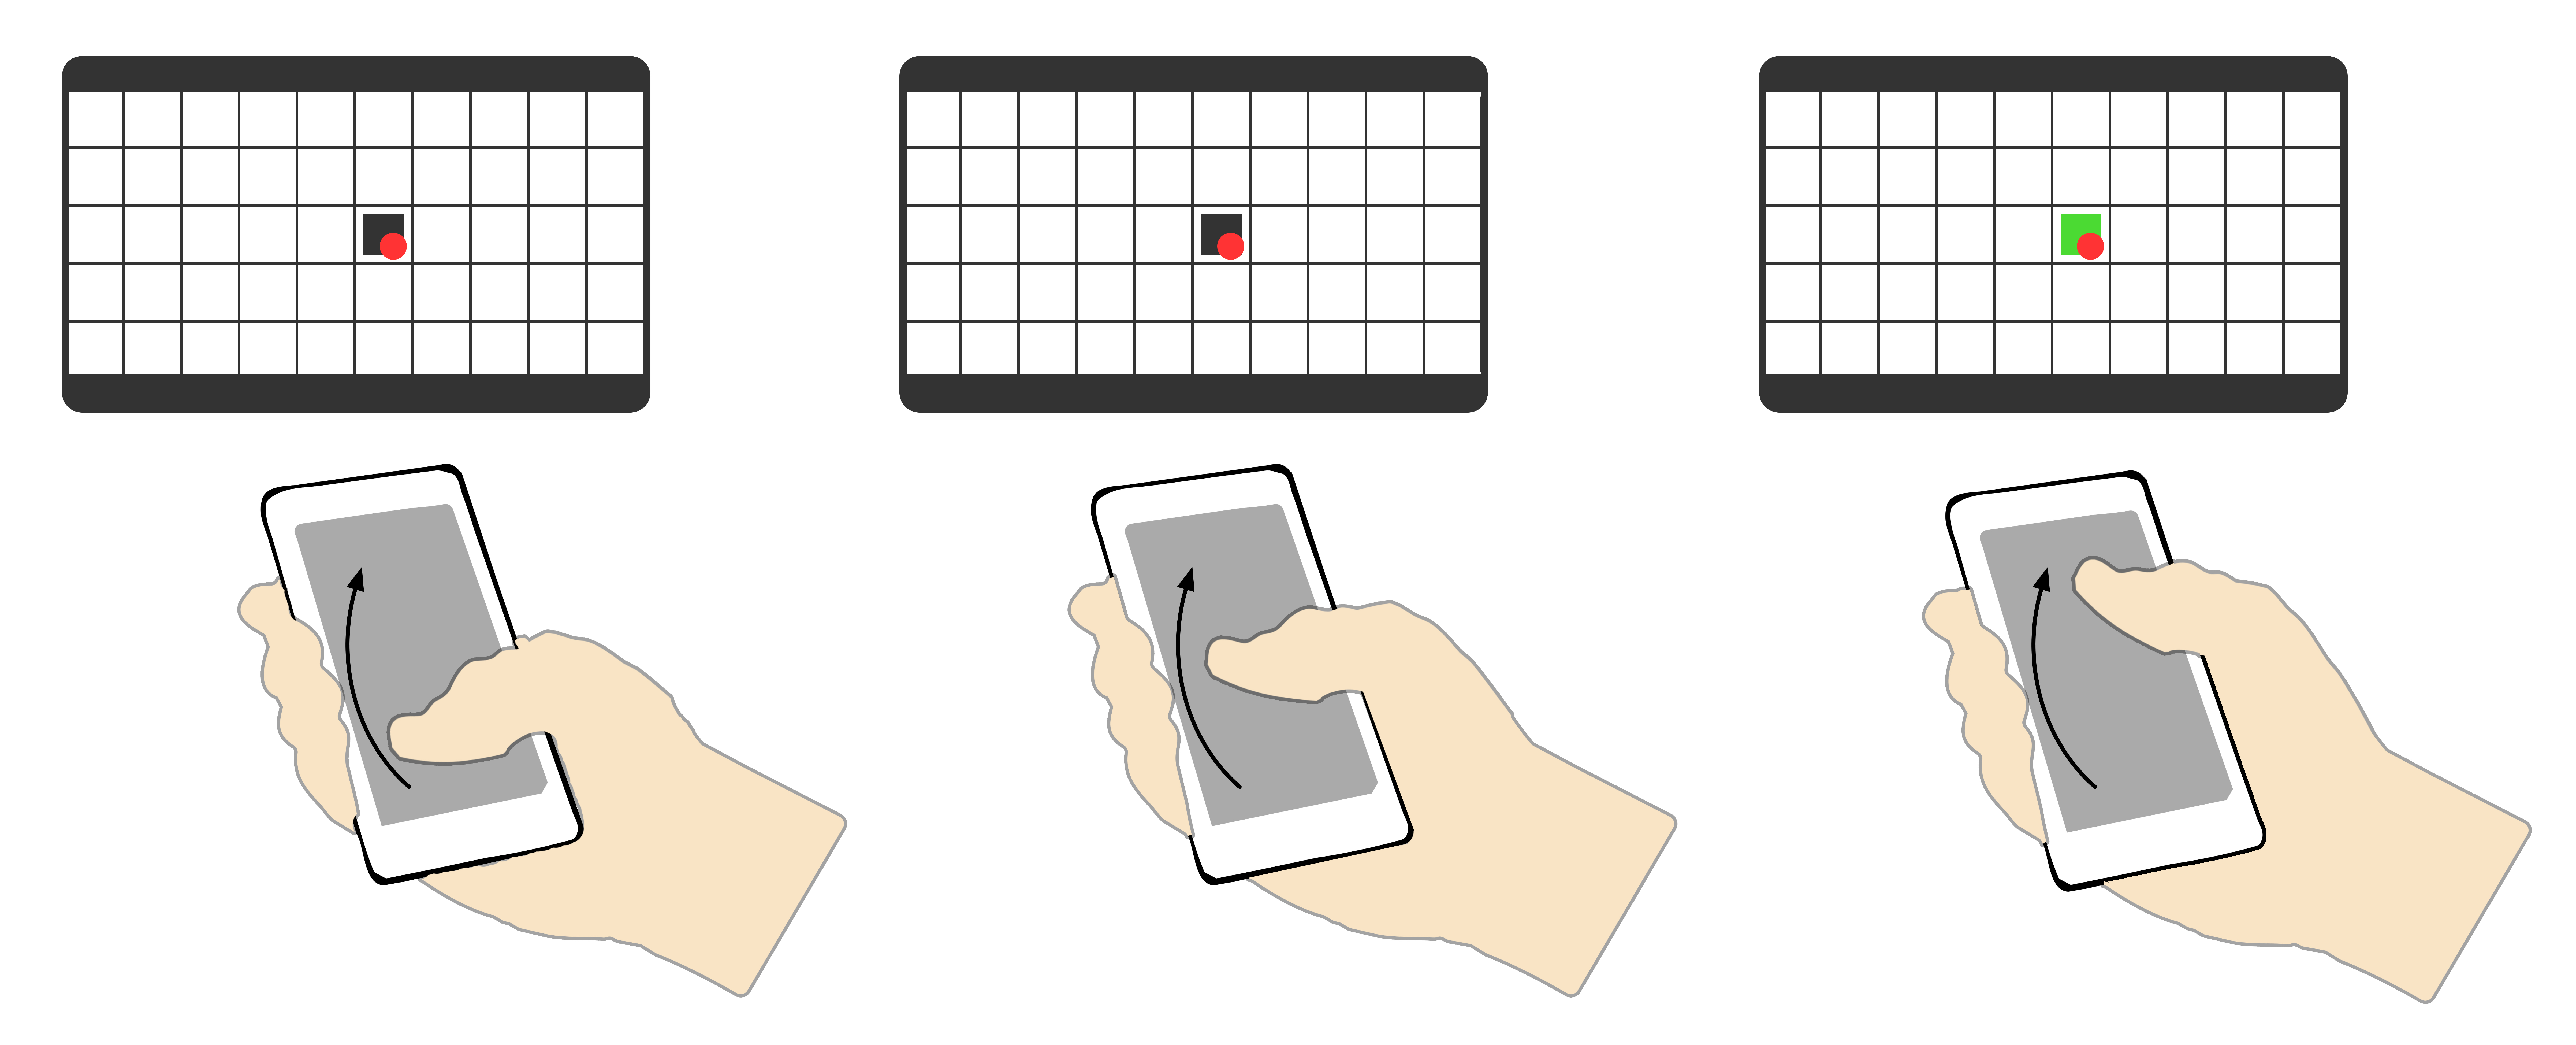
\includegraphics[width = 0.5\columnwidth]{images/swipe.jpg}\label{fig:swipeTechnique}} 
\subfloat[]{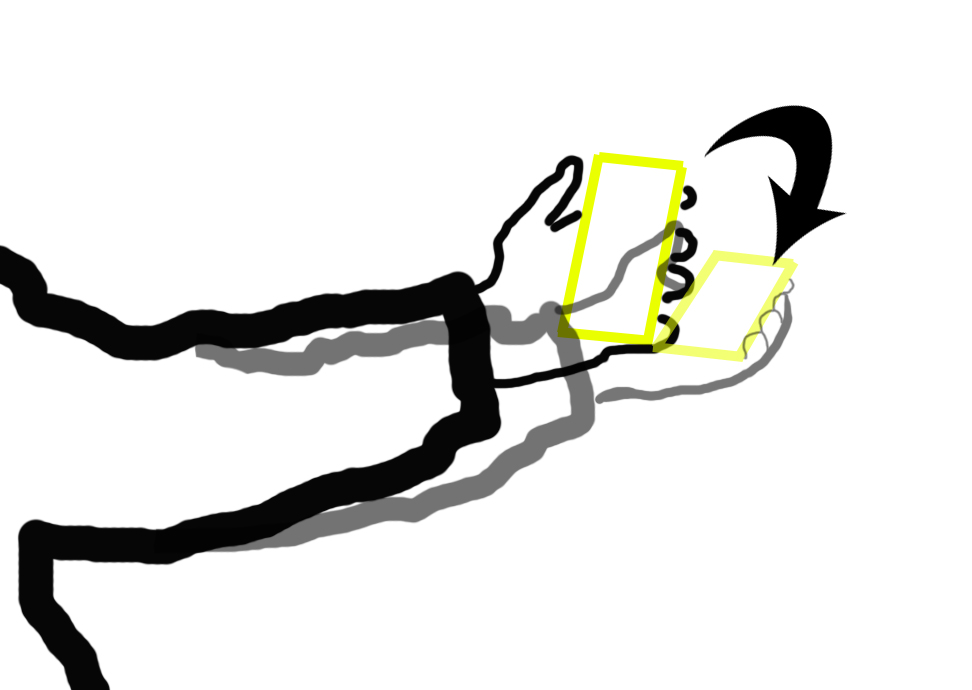
\includegraphics[width = 0.5\columnwidth]{images/tilt.jpg}\label{fig:tiltTechnique}}
\caption{
	\protect\subref{fig:swipeTechnique} The \swipe technique is performed by using the thumb to swipe;
	\protect\subref{fig:tiltTechnique} The \tilt technique is performed by doing a forward tilt motion with the phone.
}
\label{fig:swipeTilt}
\end{figure}

The \throw technique (\Cref{fig:throwTechnique}) is a combination of  
\begin{enumerate*}[label=\itshape\alph*\upshape)]
	\item{a technique for pointing \cite{Scheible:2008} i.e. using a hand as a cursor in mid-air, and}
	\item{a throw technique described by Walter et al. \cite{Walter:2014} and used in a system for sharing information on large public displays.}
\end{enumerate*}
The \throw technique is performed by 
\begin{enumerate*}[label=\itshape\roman*\upshape)]
	\item{pointing at a target on the large display with one hand (\cref{fig:throwTechnique1})} 
	\item{holding the phone in the other hand, and}
	\item{making a swinging motion towards the large display (\cref{fig:throwTechnique2}).}
\end{enumerate*}

\begin{figure}
\subfloat[]{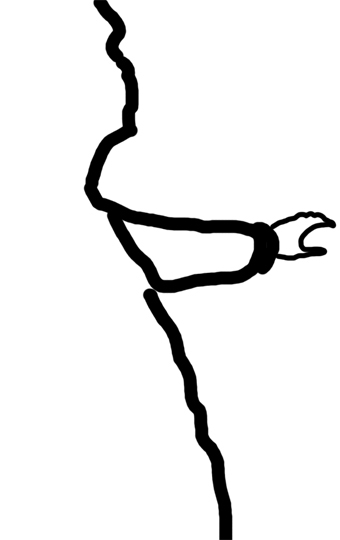
\includegraphics[width = 0.48\columnwidth]{images/throw1.jpg}\label{fig:throwTechnique1}}
\hspace{0.02\columnwidth} 
\subfloat[]{
\includegraphics[width = 0.48\columnwidth]{images/throw2.jpg}\label{fig:throwTechnique2}}
\caption{
	\protect\subref{fig:throwTechnique1} First step of \throw is to point at the screen; 
	\protect\subref{fig:throwTechnique2} Second step is to make a throwing motion in the direction of the screen.
}
\label{fig:throwTechnique}
\end{figure}

The \pinch technique (\Cref{fig:pinchTechnique}) is used in \cite{Ikematsu:2015} by Ikematsu et al., as part of a drag-and-drop method for moving data objects between devices.
Chen et al. uses a pinching gesture in \cite{Chen:2014} for cross-device interaction between a smartphone and a smartwatch to control volume. 
In \cite{Benko:2010}, Benko and Wilson used the \pinch technique for interacting with an omnidirectional dome.
This technique is again a combination of the pointing technique used by Scheible et al. and the aforementioned pinching techniques. 
The \pinch technique is performed by 
\begin{enumerate*}[label=\itshape\roman*\upshape)]
	\item{holding the phone in one hand and making a pinch gesture on the phone with the other hand (\Cref{fig:pinchTechnique1} 1), subsequently closing the hand}
	\item{pointing at a target on the large display with the closed hand (\cref{fig:pinchTechnique1} 2), and}
	\item{opening the hand to complete the technique (\cref{fig:pinchTechnique2} 3).}
\end{enumerate*}

\begin{figure}
\subfloat[]{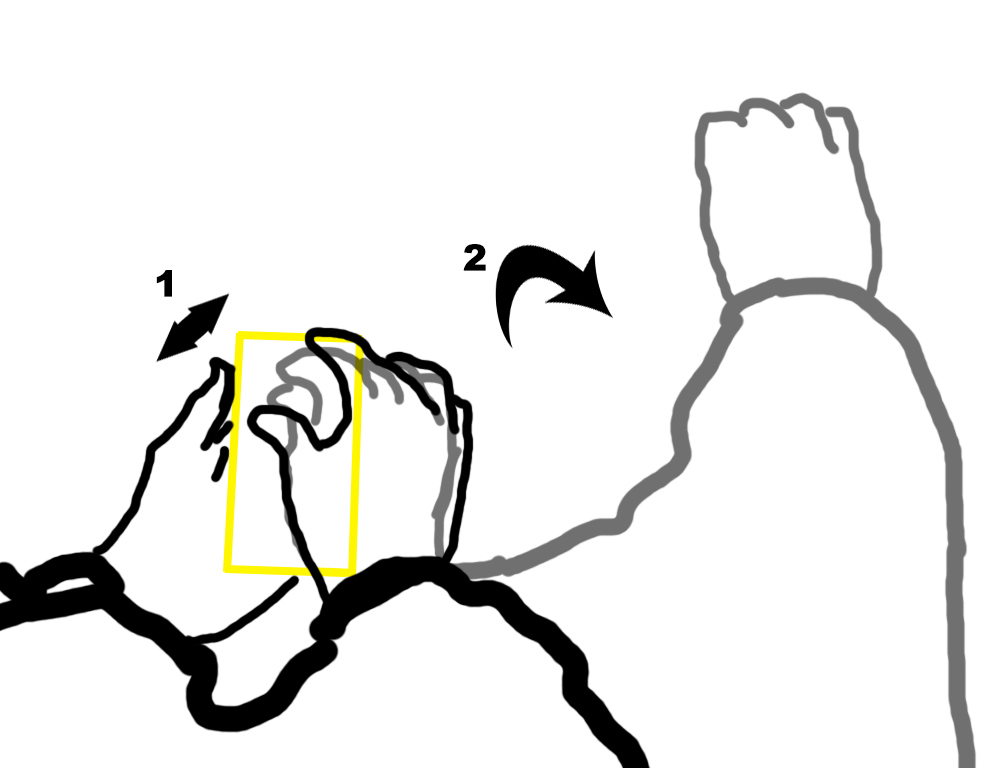
\includegraphics[width = 0.48\columnwidth]{images/pinch1.jpg}\label{fig:pinchTechnique1}}
\hspace{0.02\columnwidth}  
\subfloat[]{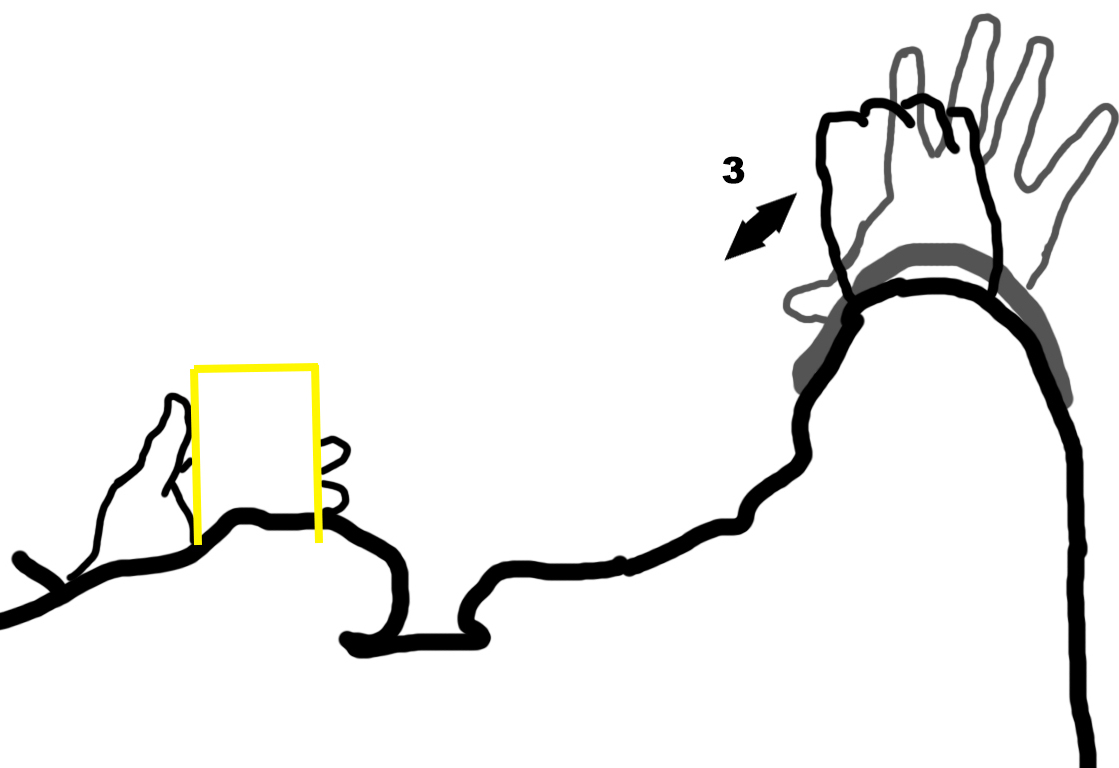
\includegraphics[width = 0.48\columnwidth]{images/pinch2.jpg}\label{fig:pinchTechnique2}}
\caption{
	\protect\subref{fig:pinchTechnique1} First step of the \pinch technique is to make a pinch gesture on the phone using the index finger and thumb. Second step is to move and use the pinched hand as a pointer; 
	\protect\subref{fig:pinchTechnique2} Third step is to release by opening the hand. 
}
\label{fig:pinchTechnique}

Our four techniques all make use of some combination of air pointing and touch gestures on the smartphone screen.
Air pointing is achieved by using the Microsoft Kinect for Windows which uses a depth camera making it possible to track a user's hand in mid-air.
A smartphones has an accelerometer and a touchscreen, former making it possible to detect motion input and the latter makes it possible to detect contact between e.g. a finger and the screen.
These technologies are, in combination with each other, used to recognize the four techniques described in this section. 
\end{figure}